\chapter{Overfitting}\label{chap:overfitting}

\section{Begriffserklärung}\label{sec:what-is-overfitting}

Genaue Daten über Krankheitsbefälle im Agrarsektor sind rar, da diese in der Regel nicht öffentlich zugänglich sind.\footnote{Datenschutz kann ein Grund dafür sein.}  Daher musste mit \textit{Overfitting} gerechnet werden. Das künstliche neurale Netzwerk soll daraufhin trainiert werden, dass es möglichst alle Befälle, die untersucht werden, erkennt. Dafür wird es im ersten Schritt mit einem Trainingsdatensatz trainiert. Im folgenden Schritt mit einem kleineren Validierungsdatensatz überprüft, wie gut das Netz trainiert wird. Overfitting tritt auf, wenn das Netz auf die Daten aus dem Trainingsdatensatz mit sehr hoher Erfolgsquote erkennt, jedoch vergleichsweise schlechte Ergebnisse bei der Validierung bzw. bei unbekannten Daten erzielt. 
\\\\
\begin{figure}[ht]
  \centering
  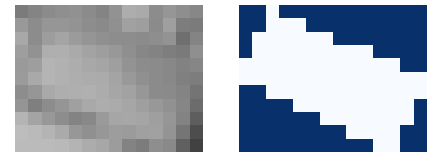
\includegraphics[height=2.5cm]{pics/mask.png}
  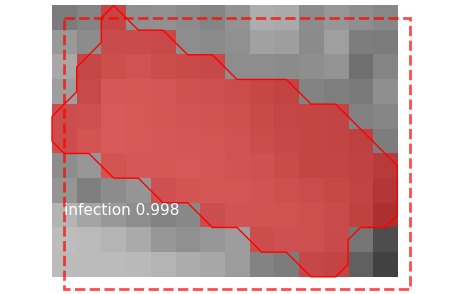
\includegraphics[height=2.5cm]{pics/pred.png}
  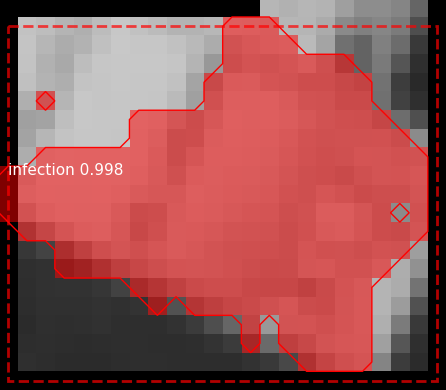
\includegraphics[height=2.5cm]{pics/bad-pred.png}
  \caption[Beispiel Overfitting]{V.l.n.r. Bild von infizierter Agrarfläche aus Trainingsdatensatz / Binärmaske der inifizierten Region, wird gemeinsam mit dem linken Bild zum Training in das KNN gespeist / Selbiges Bild, Ergebnis nach Trainingsdurchlauf, prognostizierte Ergebnisfläche in rot / Bild der selben Fläche, was nicht aus dem Trainingsdatensatz stammt, prognostizierte Ergebnisfläche in rot}
  \label{fig:example-overfitting}
\end{figure}
\noindent
\todo{Erwähnen, dass Mask RCNN Bild und Masken für Training benötigt.}
In Abb. \ref{fig:example-overfitting} ist ein Beispiel wie Overfitting sich auswirken kann. Die linken zwei Bilder sind ein exemplarischer Auszug aus dem Trainingsdatensatz. Einmal eine visuelle Repräsentation der NDVI-Werte der infizierten Agrarfläche und die Binärmaske, welche die infizierte Fläche markiert. Das selbe Bild wurde nach einem erfolgreichen Trainingsdurchlauf der Mask R-CNN-Implementierung übergeben und es hat den erkrankten Bereich nahezu perfekt erkannt. Das vierte Bild zeigt zentriert das selbe Feld. Jedoch ist der Ausschnitt größer, rotiert und die Aufnahme stammt von einem anderen Datum.\todo{Genaues Datum nötig?} Der Prognose zur Folge ist die Infizierung auf die benachbarten Felder übergesprungen, was nicht der Wahrheit entspricht. Overfitting ist ein bekanntes Problem im Bereich des maschinellen Lernens und es existieren multiple Methoden, um dem entgegenzuwirken.